\documentclass[tikz]{standalone}
\usepackage{pgfplots}

\pgfplotsset{
	compat = 1.8
}

\begin{document}

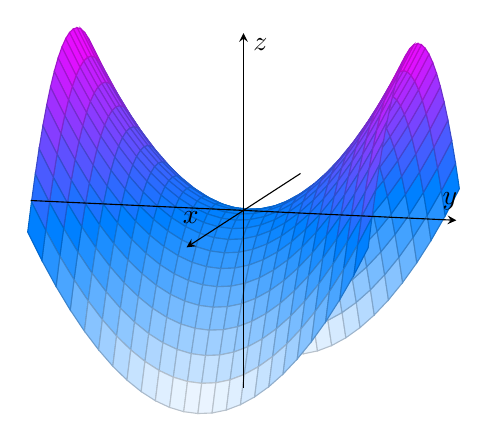
\begin{tikzpicture}
\begin{axis}[
    view = {105}{10},
	axis equal,
	axis lines = center,
	xmin=-2.5, xmax=2.5, ymin=-2.5, ymax=2.5,
    xlabel={$x$},ylabel={$y$},zlabel={$z$},
    ticks = none,
    colormap/cool,
    set layers
]
\addplot3[
	surf,
    domain=-2:2,y domain=-2:2,
    z buffer=sort,
    on layer = axis background
    ]
    ({x}, {y}, {0.5*(-x^2 + y^2)});
]
\end{axis}
\end{tikzpicture}

\end{document}